\documentclass[conference]{IEEEtran}
\IEEEoverridecommandlockouts
% The preceding line is only needed to identify funding in the first footnote. If that is unneeded, please comment it out.
\usepackage{cite}
\usepackage{amsmath,amssymb,amsfonts}
\usepackage{algorithmic}
\usepackage{caption}
\usepackage{subcaption}
% \usepackage{subfigure}
\usepackage{graphicx}
\usepackage{textcomp}
\usepackage{xcolor}
\usepackage{graphicx}
\usepackage[colorinlistoftodos]{todonotes}
\def\BibTeX{{\rm B\kern-.05em{\sc i\kern-.025em b}\kern-.08em
    T\kern-.1667em\lower.7ex\hbox{E}\kern-.125emX}}
\begin{document}

\title{Optimize Configuration For Mismatched PV System}
\author{\IEEEauthorblockN{Dafang Zhao, Fukuhito Ooshita, and Michiko Inoue}
%Email: 
\IEEEauthorblockA{Nara Institute of Science and Technology, Japan\\
% Win : My email is @ku.th, Not @ku.ac.th
Email:   \{zhao.dafang.yu7, f-ooshita, kounoe\}@is.naist.jp}}
\maketitle

\begin{abstract}
Power generation efficiency of Photovoltaic(PV) system are significantly affected by partial shading and solar cell damage. This efficiency loss caused by turning on bypass diode of PV panels, which we called mismatch loss. By using some reconfiguration technology to reconfigure electrical series or parallel connection can reduce the mismatch loss and maximize power generation. Recently, an efficient reconfiguration method is proposed. This method applies precise power simulations based on a list of configuration candidates. However, some of the configuration candidates are not be able to realized and this method does not show any systematic way to identify such feasibility. Thus, in this paper we propose a very fast algorithm to check feasibility and reduce wiring complexity.
\end{abstract}

% \begin{IEEEkeywords}
% component, formatting, style, styling, insert
% \end{IEEEkeywords}

\section{Introduction}
With fossil depleting and the pollution of the environment becomes more serious. Green and renewable energy have become necessary for a sustainable society and environment. Photovoltaic(PV) receive significant attention since it has unlimited energy and can be easily scaled up. However, due to the nature of photovoltaic cell structure, PV arrays are sensitive to partial shading and PV cell fault or aging. That means when PV cells or modules experience different irradiance or do not uniformly generate power, the PV array is mismatched and unable to efficiently generate power. Additionally, when PV array under mismatch condition it will accelerate aging and heating for PV cells. That will cause a short circuit of PV array for further damaging. In order to prevent damaging on PV array and maximize power generation many reconfiguration method been proposed.

A PV panel level reconfiguration using genetic algorithm (GA) is proposed in \cite{carotenuto2015evolutionary}. Though it can give a new configuration, but computing cost is significant and algorithm cannot generate the best configuration precisely. The work in \cite{nguyen2008adaptive} proposed a switch matrix to reconfigure shadowed PV array, but it can not be able to apply on large size PV array. Paper \cite{storey2013improved} using "irradiance level equalization" method to dynamic reconfigure PV array and improve power generation efficiency over 10\%. The work in \cite{malathy2017reconfiguration} employed Irradiation equivalence method by using swathing matrix relocate PV panels. At PV module level, paper \cite{wang2014architecture} proposed a dynamic programming algorithm to adaptively produce near-optimal reconfiguration, the work in \cite{storey2014optimized} proposed a method for dynamic reconfigure PV array based on string-configured topology.
Fig.\ref{compare} shows the difference of shadowed PV array between only using Global maximum point tracking method and using reconfiguration strategy.
% finding global maximum point tracking (without reconfiguration) 
% and reconfigured PV array.
It puts into evidence that after reconfiguration shadowed PV array be able to generate more power and P—V curve has only one peak which is very useful for maximum point tracking devices.

To give the reconfiguration more expeditiously, the mathematical searching algorithm needs to be developed instead of sample exhaustive searching algorithm. Reference \cite{faldella1991architectural} given a method based on the tabular searching algorithm, it performing well on small size PV array, but it is hard to apply on a large scale array. Paper \cite{iraji2017optimisation} proposed an algorithm based on particle swarm optimisation to find switch matrix topology. 

But the reference \cite{carotenuto2015evolutionary} -\cite{iraji2017optimisation} given reconfiguration methods either force on uniformly distributed shadow or using GA and exhaustive searching algorithm. Reference \cite{orozco2016optimized} developed a fast reconfiguration strategy by using approximated values of MPP current and voltage to generate configuration candidates. In this strategy, first list and calculate configuration candidates by a fast estimation method in \cite{orozco2015fast}, and for each candidate, precise power simulation are applied. However, when the size of PV array are extremely large, it's impossible to do power simulation for each configuration candidate, and some configuration candidates might not be feasible, this is, it is impossible to realize a configuration designed by given PV panels.

In this paper, we propose an algorithm to identify feasibility based on the configuration candidates from \cite{orozco2016optimized} and a new connection topology to increase system flexibility without loss too much accuracy. The layout of reaming sections as below. Section \ref{Sec2} illustrate the model setting of PV array and etc.. Section \ref{Sec3} give the details of configuration candidates from \cite{orozco2016optimized}. Section\ref{Sec4} is the definition of feasibility. Section \ref{Sec5} and \ref{Sec6} give the details of algorithm and evaluation. Section \ref{Sec7} is the simulation result. Conclusions are provided in the last section.
% By reconfigure electrical connection of mismatched PV array can increase power generation efficiency. 
\begin{figure}
    \centering
    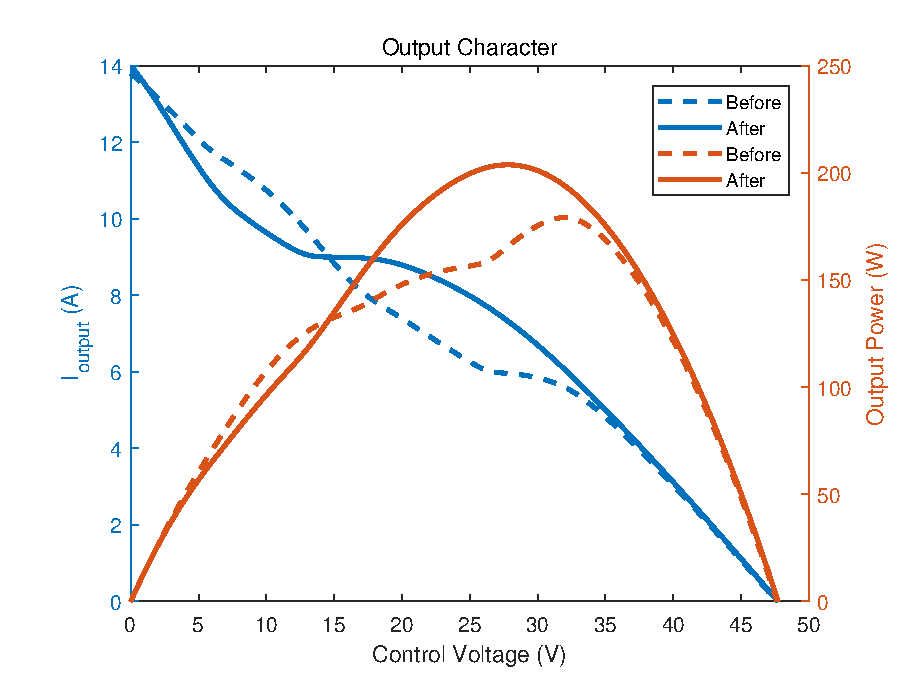
\includegraphics[width=0.8\linewidth]{compare.eps}
    \caption{Maximum Power generation difference between before and after reconfiguration}
    \label{compare}
\end{figure}

\section{Photovoltaic array}\label{Sec2}
In this paper we use the following model of PV array, module, string and panel as showed in Fig.\ref{model}. In general, a PV array is a combination of multiple PV panels. Several series-connected PV panels in formed of a string. And several parallel connected string in formed of PV array. This is typical S-P network PV array. A PV panel usually formed by three series-connected PV module which in formed of several series-connected PV cells. For each PV module a bypass diode is connected in parallel for reversing the reverse current. PV cells in a PV panel may have different conditions (irradiance or fault) and hence have different  upper limits for their generated currents. Therefore, as shown in Fig.\ref{one_panel} for lower control voltage, only PV cells can generate high currents be able to work and other PV cells don't generate current with their bypass diode turned on. Fig.\ref{ser-par} show I-V character for two series and parallel connected PV panels. The series-connection structure accepts a wider range of control voltage and parallel-connection structure can generate higher current.
\begin{figure}
    \centering
    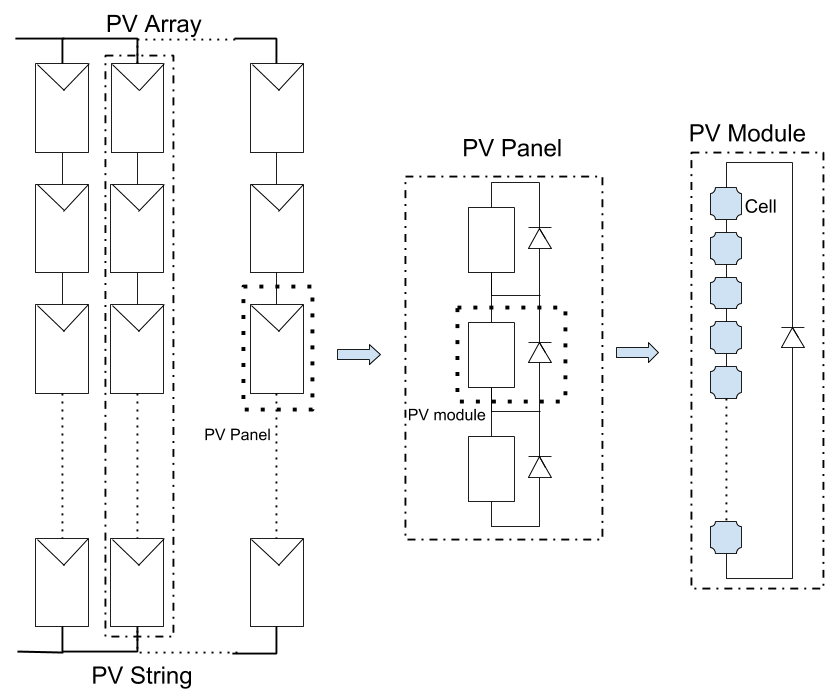
\includegraphics[width=0.8\linewidth]{module.png}
    \caption{PV array, string, module and panel}
    \label{model}
\end{figure}
When understanding the I-V characteristics of different structure of PV panels, by using the algorithm in \cite{carotenuto2014online} we can find the I-V curves of panels and (near) MPPs, short circuit current, open circuit voltage of each panel in mismatch condition. These values form a fingerprint of connection.
\begin{figure}
     \centering
     \begin{subfigure}[b]{0.8\linewidth}
         \centering
         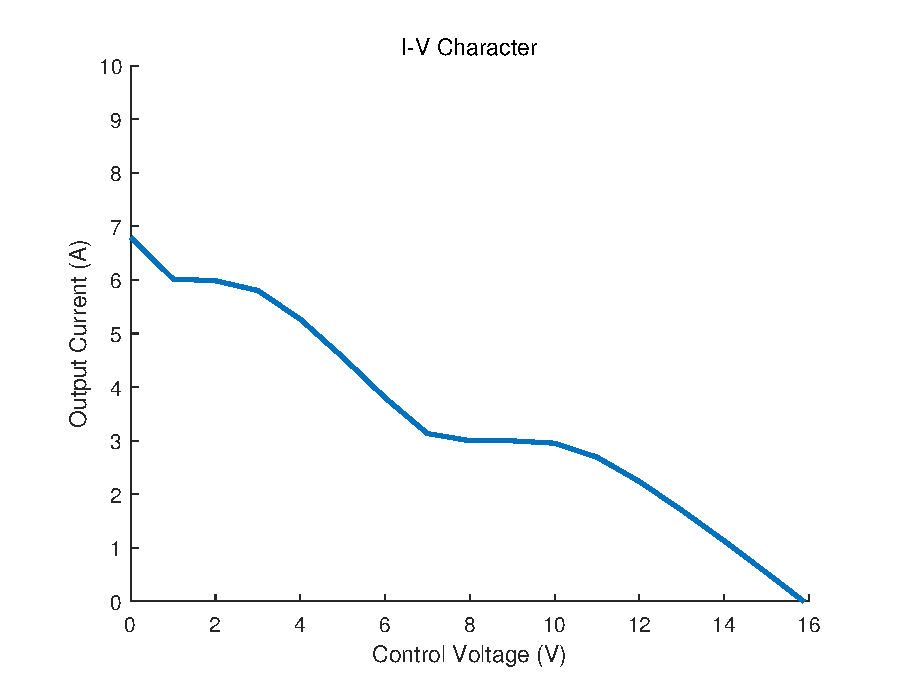
\includegraphics[width=\linewidth]{IEEE_CEC_SS/one-panel.eps}
         \caption{I-V characteristics on different control voltage}
         \label{one_panel}
     \end{subfigure}
     \hfill
     \begin{subfigure}[b]{0.8\linewidth}
         \centering
         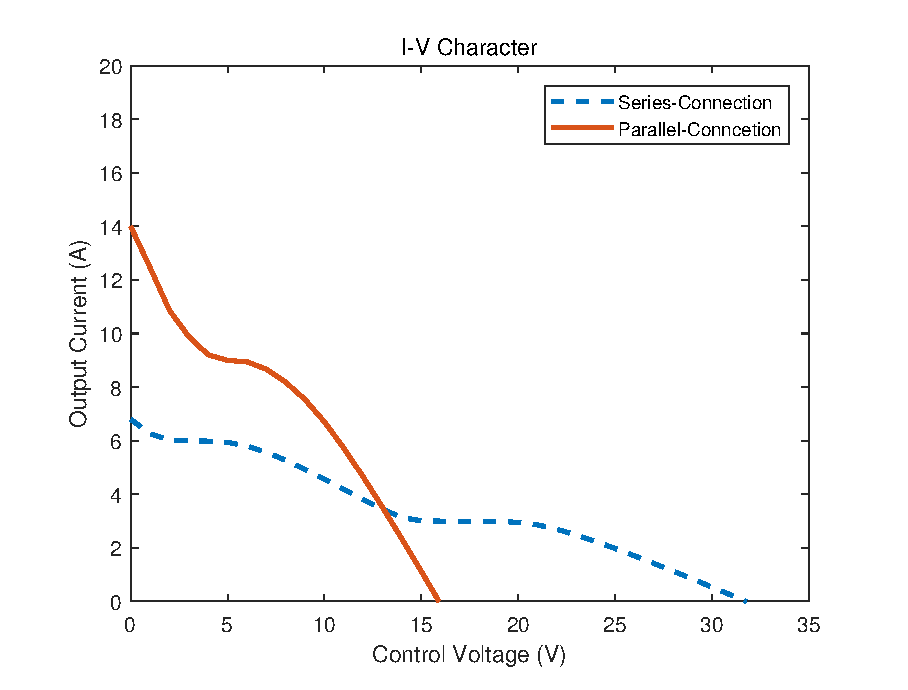
\includegraphics[width=\linewidth]{IEEE_CEC_SS/ser-par.eps}
         \caption{Series and parallel connection I-V character}
         \label{ser-par}
     \end{subfigure}
        \caption{PV Panel I-V characteristic}
        \label{fig:three graphs}
\end{figure}
\section{Related works}\label{Sec3}

\section{Feasibility}\label{Sec4}

\section{An algorithm to identify feasibility}\label{Sec5}

\section{Evaluation of optimization algorithm}\label{Sec6}

\section{Simulation}\label{Sec7}

\section*{Acknowledgment}


% \section*{References}

\renewcommand\refname{Reference}
\bibliographystyle{ieeetr}
\bibliography{reference}
% \begin{thebibliography}{00}
% \bibitem{b1} G. Eason, B. Noble, and I. N. Sneddon, ``On certain integrals of Lipschitz-Hankel type involving products of Bessel functions,'' Phil. Trans. Roy. Soc. London, vol. A247, pp. 529--551, April 1955.
% \bibitem{b2} J. Clerk Maxwell, A Treatise on sdElectricity and Magnetism, 3rd ed., vol. 2. Oxford: Clarendon, 1892, pp.68--73.
% \bibitem{b3} I. S. Jacobs and C. P. Bean, ``Fine particles, thin films and exchange anisotropy,'' in Magnetism, vol. III, G. T. Rado and H. Suhl, Eds. New York: Academic, 1963, pp. 271--350.
% \bibitem{b4} K. Elissa, ``Title of paper if known,'' unpublished.
% \bibitem{b5} R. Nicole, ``Title of paper with only first word capitalized,'' J. Name Stand. Abbrev., in press.
% \bibitem{b6} Y. Yorozu, M. Hirano, K. Oka, and Y. Tagawa, ``Electron spectroscopy studies on magneto-optical media and plastic substrate interface,'' IEEE Transl. J. Magn. Japan, vol. 2, pp. 740--741, August 1987 [Digests 9th Annual Conf. Magnetics Japan, p. 301, 1982].
% \bibitem{b7} M. Young, The Technical Writer's Handbook. Mill Valley, CA: University Science, 1989.

% \end{thebibliography}

\end{document}
